%\documentclass[sigplan,review,nonacm,10pt]{acmart}
\documentclass[sigplan,nonacm,10pt]{acmart}

\usepackage{minted}
\usepackage{makecell}
\usepackage{booktabs}
\usepackage{microtype}
\graphicspath{ {./figs/} }
\newcommand\aste{%
$^{(\ast)}$
}
\usepackage[subtle]{savetrees}

% https://tex.stackexchange.com/questions/655620/how-to-make-acmart-stop-complaining-about-missing-country-in-affiliation
\makeatletter
\def\@ACM@checkaffil{% Only warnings
    \if@ACM@instpresent\else
    \ClassWarningNoLine{\@classname}{No institution present for an affiliation}%
    \fi
    \if@ACM@citypresent\else
    \ClassWarningNoLine{\@classname}{No city present for an affiliation}%
    \fi
    \if@ACM@countrypresent\else
        \ClassWarningNoLine{\@classname}{No country present for an affiliation}%
    \fi
}
\makeatother

%%
%% \BibTeX command to typeset BibTeX logo in the docs
\AtBeginDocument{%
  \providecommand\BibTeX{{%
    Bib\TeX}}}

%% Rights management information.  This information is sent to you
%% when you complete the rights form.  These commands have SAMPLE
%% values in them; it is your responsibility as an author to replace
%% the commands and values with those provided to you when you
%% complete the rights form.
\setcopyright{acmcopyright}
\copyrightyear{2023}
\acmYear{2023}
%\acmDOI{XXXXXXX.XXXXXXX}

%% These commands are for a PROCEEDINGS abstract or paper.
\acmConference[CS294]{CS294}{Fall 2023}{Berkeley, CA}
%%
%%  Uncomment \acmBooktitle if the title of the proceedings is different
%%  from ``Proceedings of ...''!
%%
%%\acmBooktitle{Woodstock '18: ACM Symposium on Neural Gaze Detection,
%%  June 03--05, 2018, Woodstock, NY}
%\acmPrice{15.00}
%\acmISBN{978-1-4503-XXXX-X/18/06}


%%
%% Submission ID.
%% Use this when submitting an article to a sponsored event. You'll
%% receive a unique submission ID from the organizers
%% of the event, and this ID should be used as the parameter to this command.
%%\acmSubmissionID{123-A56-BU3}

%%
%% For managing citations, it is recommended to use bibliography
%% files in BibTeX format.
%%
%% You can then either use BibTeX with the ACM-Reference-Format style,
%% or BibLaTeX with the acmnumeric or acmauthoryear sytles, that include
%% support for advanced citation of software artefact from the
%% biblatex-software package, also separately available on CTAN.
%%
%% Look at the sample-*-biblatex.tex files for templates showcasing
%% the biblatex styles.
%%

%%
%% The majority of ACM publications use numbered citations and
%% references.  The command \citestyle{authoryear} switches to the
%% "author year" style.
%%
%% If you are preparing content for an event
%% sponsored by ACM SIGGRAPH, you must use the "author year" style of
%% citations and references.
%% Uncommenting
%% the next command will enable that style.
%%\citestyle{acmauthoryear}
\settopmatter{printacmref=false}

%%
%% end of the preamble, start of the body of the document source.
\begin{document}

%%
%% The "title" command has an optional parameter,
%% allowing the author to define a "short title" to be used in page headers.
% \title{TidalSim: Mixing Functional Simulation, $\mu$Arch Models, and RTL Simulation for Rapid Microarchitectural Iteration and Evaluation}
\title{TidalSim: Multi-Level Simulation for Rapid Microarchitectural Iteration and Evaluation}

%%
%% The "author" command and its associated commands are used to define
%% the authors and their affiliations.
%% Of note is the shared affiliation of the first two authors, and the
%% "authornote" and "authornotemark" commands
%% used to denote shared contribution to the research.

\author{\href{https://orcid.org/0000-0001-6934-6577}{Vighnesh Iyer}, Raghav Gupta, Dhruv Vaish, Young-Jin Park, Charles Hong, Sophia Shao, \href{https://orcid.org/0000-0003-2324-1715}{Borivoje Nikolić}}
\email{{vighnesh.iyer,rgupta,dvaish,bora}@berkeley.edu}
\affiliation{%
  \institution{UC Berkeley}
}

% \author{Borivoje Nikolić}
% \email{bora@eecs.berkeley.edu}
% \orcid{0000-0003-2324-1715}
% \affiliation{%
%   \institution{UC Berkeley}
% }


%%
%% By default, the full list of authors will be used in the page
%% headers. Often, this list is too long, and will overlap
%% other information printed in the page headers. This command allows
%% the author to define a more concise list
%% of authors' names for this purpose.
\renewcommand{\shortauthors}{Iyer, Vighnesh et al.}

\begin{abstract}

% Due to the end of Moore's law and Dennard scaling...
% lol no

Existing approaches to microarchitecture simulation cannot simultaneouly deliver the three goals of high throughput, low latency, and high fidelity.
Rapid RTL-level microarchitectural iteration and evaluation on real applications is enabled by a simulator that can meet these three objectives.
Our multi-level simulator combines functional ISA-level simulation, microarchitectural warmup models, and RTL simulation to produce accurate IPC traces.
This new paradigm of multi-level simulation opens the door to an efficient and accurate DSE methodology, rapid evaluation of RTL-level optimizations, and automatic extraction of RTL-level traces of interesting and unique segments of long workloads.

\end{abstract}

% \received{20 February 2007}
% \received[revised]{12 March 2009}
% \received[accepted]{5 June 2009}

\maketitle

\section{Introduction}

% Fill only the first page
% 1. Describe the problem
%   use an example to introduce the problem, consider this scenario..., how would you evaluate it?
% 2. State your contributions
%   write as a bulleted list, make the contributions refutable, make them specific
%   each claim that we make should contain a forward reference to a section that provides evidence for that claim

% What is the typical microarchitectural design and iteration process?
Designing a microprocessor involves evaluating a proposed microarchitecture on representative workloads, and optimizing the microarchitecture to meet the power, performance, and area targets for a set of applications based on your target market.
Evaluation of a microarchitecture is typically a lengthy process and these long evaluation cycles bottleneck the iteration loop of making a microarchitectural change and seeing its impact.
The agile design of microprocessors demands an evaluation methodology with low latency that enables rapid microarchitectural development, optimization, and tuning.

\subsection{The Problem}

% What workloads do we use to evaluate our decisions?
Consider this scenario: you (a microarchitect) are designing a next-generation microprocessor for a mobile SoC optimized for web browsing, and you want to make changes to improve the PPA of your design.
Microarchitects rarely start completely from scratch; instead, you have the RTL from the previous generation's microprocessor, a functional ISA-level model, and perhaps a performance model.
Let's say you also have representative web and mobile applications and perhaps some smaller benchmark suites from the software engineering side.

The microarchitecture iteration loop involves making changes to the RTL, evaluating them for correctness and performance on the real-world applications the SoC will see, and using the evaluation results (e.g. performance metrics, identified bottlenecks, profiling traces, RTL-level waveforms) to guide further microarchitectural exploration (see Figure \ref{fig:uarch_iteration_loop}).

\begin{figure}
  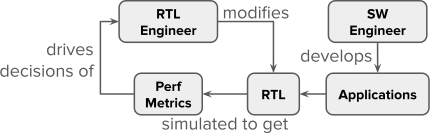
\includegraphics[width=\linewidth]{dynamic/tidalsim/uarch_iteration_flow.pdf}
  \caption{Typical microarchitecture iteration loop}
  \label{fig:uarch_iteration_loop}
\end{figure}

% Want to consider 1) evaluation of a new microarchitectural structure, 2) optimizing the uArch of a given structure, 3) tuning hardware parameters.
% What kinds of decisions do we want to make during the process?
There are broadly three categories of RTL changes you might make:
\begin{enumerate}
  % Evaluate the usefulness of the structure, what new state is needed
  \item Creating a completely new structure (e.g. a vector unit, a prefetcher, a new type of branch predictor)
  % Optimization of the uArch e.g. reordering support, multiple dispatch and parallelism
  \item Optimizing the microarchitecture of an existing structure or pipeline (e.g. reducing the dispatch latency from the ROB, adding a new forwarding path)
  % Parameter tuning and its impact on performance
  \item Parameterizing an RTL unit or tuning hardware parameters that already exist (e.g. tuning cache hierarchy and sizing, queue sizing in the LSU)
\end{enumerate}

For the latter two types of RTL changes, the bottleneck in their evaluation is often not the architectural modeling, RTL development, or verification, but rather measuring the impact of the changes on real workloads.
If you only had access to traditional simulation techniques, you would be stuck with these options:
\begin{itemize}
  \item `Fast' but low startup latency simulators (functional and architectural models) which would lead to decisions being made based on likely inaccurate data
  \item `Fast' but high startup latency simulators (FPGA-based simulators) which would bottleneck the speed of microarchitectural iteration
  \item `Slow` simulators (RTL simulators) that would not be able to run a full workload to begin with in a reasonable time
\end{itemize}

You would like the best of all worlds: a simulator that is fast (high throughput to run real workloads), has low startup latency (to get performance results from a proposed change quickly), and is accurate (so you can make microarchitectural decisions confidently).

% I want this table to show up on the second page!
\begin{figure*}[!hbt]
  \small
  % Alladin (analytical models, often specialized for kernel accelerators), functional ISA simulation, gem5-style perf sim (this is the most diverse category), RTL sim, FPGA prototype (high fidelity if IO modeling isn't an issue), FPGA emulator (Firesim), Emulation (Palladium)
  \begin{tabular}{>{\raggedright\arraybackslash}p{2cm}>{\raggedright\arraybackslash}p{3cm}>{\raggedright\arraybackslash}p{2cm}>{\raggedright\arraybackslash}p{3cm}>{\raggedright\arraybackslash}p{3cm}>{\raggedright\arraybackslash}p{2cm}}\toprule
  \textbf{Abstraction} & \textbf{Primitives} & \textbf{Simulation} & \textbf{Examples} & \textbf{Utility} & \textbf{Domain} \\\midrule
  %Transistor-level & PDK transistor models, wires, passives, physical geometry & Solving systems of differential equations & SPICE, Spectre & Analog circuit design, standard cell characterization & Continuous time and voltage\\\midrule
  Gate-level & PDK standard cells, arbitrary time advancement & Event-driven simulation & Structural Verilog with SDF annotation & Post-syn verification, timing validation & Discrete time, 4-valued state\\\midrule
  Register-transfer level & Flops, SRAMs, logic/arithmetic operators, wires & Transition system simulation & Lava\cite{lava}, Chisel\cite{chisel}, Amaranth\cite{amaranth}, PyMTL3\cite{pymtl3} & Synchronous digital circuit design and verification & Regular clock ticks, 2/4 valued signals\\\midrule
  Digital discrete-event modeling & State, event-triggered blocks, delays & Event-driven simulation & Verilog, VHDL & Behavioral modeling of digital/analog IPs & Discrete time, 4-valued signals\\\midrule
  Pipelines & Token streams, ordered operations, dataflow history & Ordered token processing & DFiant\cite{dfiant}, TL-Verilog\cite{tlverilog}, PipelineC\cite{pipelinec} & Dataflow circuits, auto-pipelining & Tokens in, tokens out\\\midrule
  Imperative control & State, update blocks, control blocks & Interpretation & Calyx\cite{calyx}, XLS\cite{xls} & High-level synthesis & Steps in the control block\\\midrule
  Transaction-level models & Ports, channels, threads, imperative code & TLM kernel & SystemC-TLM, PyMTL3 & System-level modeling, high-level synthesis & Transaction traces\\\bottomrule
  \end{tabular}
  \caption{The spectrum of simulation techniques and how they compare on various axes.}
  \label{fig:spectrum_of_simulators}
\end{figure*}

\subsection{Our Contributions}

In this paper, we propose a simulation methodology that dramatically reduces the evaluation time overhead of microarchitectural iteration.
We demonstrate:

\begin{itemize}
  \item A technique to combine functional ISA-level simulation, microarchitectural warmup models, and RTL-level simulation to produce a `multi-level' simulator capable of running at 10 MIPS with low startup latency and high accuracy (under 5\% error with respect to full RTL simulation)
  \item The ability to produce detailed IPC traces (with time-granularity of 10k instruction windows) for long running workloads (millions of dynamic instructions) in a matter of seconds
\end{itemize}

\section{Background}

% Later: I should say that all these tasks involve benchmark extraction and rapid evaluation and I can help in all of these tasks with tidalsim
% However, for this paper, I will focus on just the simulation and performance estimation aspect
There are many tasks involved in the design of a microprocessor such as architectural and performance modeling, the RTL design itself, verification, power and area estimation, and of course performance evaluation.
In this paper, we only focus on improving the latency and accuracy of performance evaluation.
The primary means of performance evaluation is simulation, so we will first survey existing simulation techniques.

\subsection{The Spectrum of Simulation Techniques}

There are many analytical, architectural, and microarchitectural simulation techniques that have been developed over the past few decades spanning the gamut on various axes:

\begin{itemize}
  \item \textbf{Throughput}: how many instructions can be simulated per real second? Often given in MIPS (Millions of Instructions Per Second).
  \item \textbf{Accuracy / fidelity}: how accurate are the output metrics of the simulator with respect to the final SoC in its real environment?
  \begin{itemize}
    % with Early stage vs late stage / exploratory vs tuning: some simulators are designed for exploring the impact of very high-level parameters while others are
    \item This axis is correlated to whether a simulator is designed for early-stage exploration of high-level parameters or for late-stage tuning of a refined microarchitecture.
  \end{itemize}
  \item \textbf{Startup latency}: how long does it take from the moment the simulator's parameters are modified to when the simulator begins executing the first simulated instruction?
  \item \textbf{Metric diversity}:  types of metrics that can be extracted
  \item - cost / compute (palladium cost is not merely indicental, but fundamental to the technique)
\end{itemize}

% Talk about simulation methodologies
% Insert table of existing methodologies

The spectrum of simulators that already exist and their limitations.

% Cite existing perf simulators: gem5, Sniper, ZSim, SST

% Don't want to design perf model and then design RTL to match that - what a waste, not agile!
% Also how much fidelity is typical from perf sims? (cite paper on arch simulators considered harmful). miscorrelation vs RTL *compounds* over simulation time!

asdf\cite{arch_sim_considered_harmful}

\subsection{Sampled Microarchitectural Simulation}

Why not just go into perf simulators? - the correlation problem gets compounded 2x - sampling error + perf sim - RTL sim correlation errors
Aren't "trends" enough? Not when we care about small IPC changes! The absolute number matters! Also what are the special things we can get from RTL simulation that perf sim can't get us?

Talk about sampled simulation and some prior work on that

\section{The Concept of Multi-Level Simulation}

Why multi-level simulation?
% Introduce the problem and your idea using *examples* and only then present the general case

For embeddings:
Binary agnostic
Microarchitecture agnostic
- BBVs - binary aware, uarch unaware
- NPS - binary unaware, uarch unaware
- BBVs + uarch features - binary aware, uarch aware
- Ideal - binary unaware, uarch aware

\section{Implementation}

\section{Results}

\section{Related Work}

\section{Conclusion}

\begin{acks}
Acks go here (Seah, Joonho, Sophia, Chris)
\end{acks}

\bibliographystyle{ACM-Reference-Format}
\bibliography{references}

% \appendix

\end{document}
\endinput
